\underbar{\textbf{\large Ejercicio 1:}} Implemente los miembros imprescindibles para que las relaciones se puedan realizar:
\begin{figure}[h]
  \begin{center}
    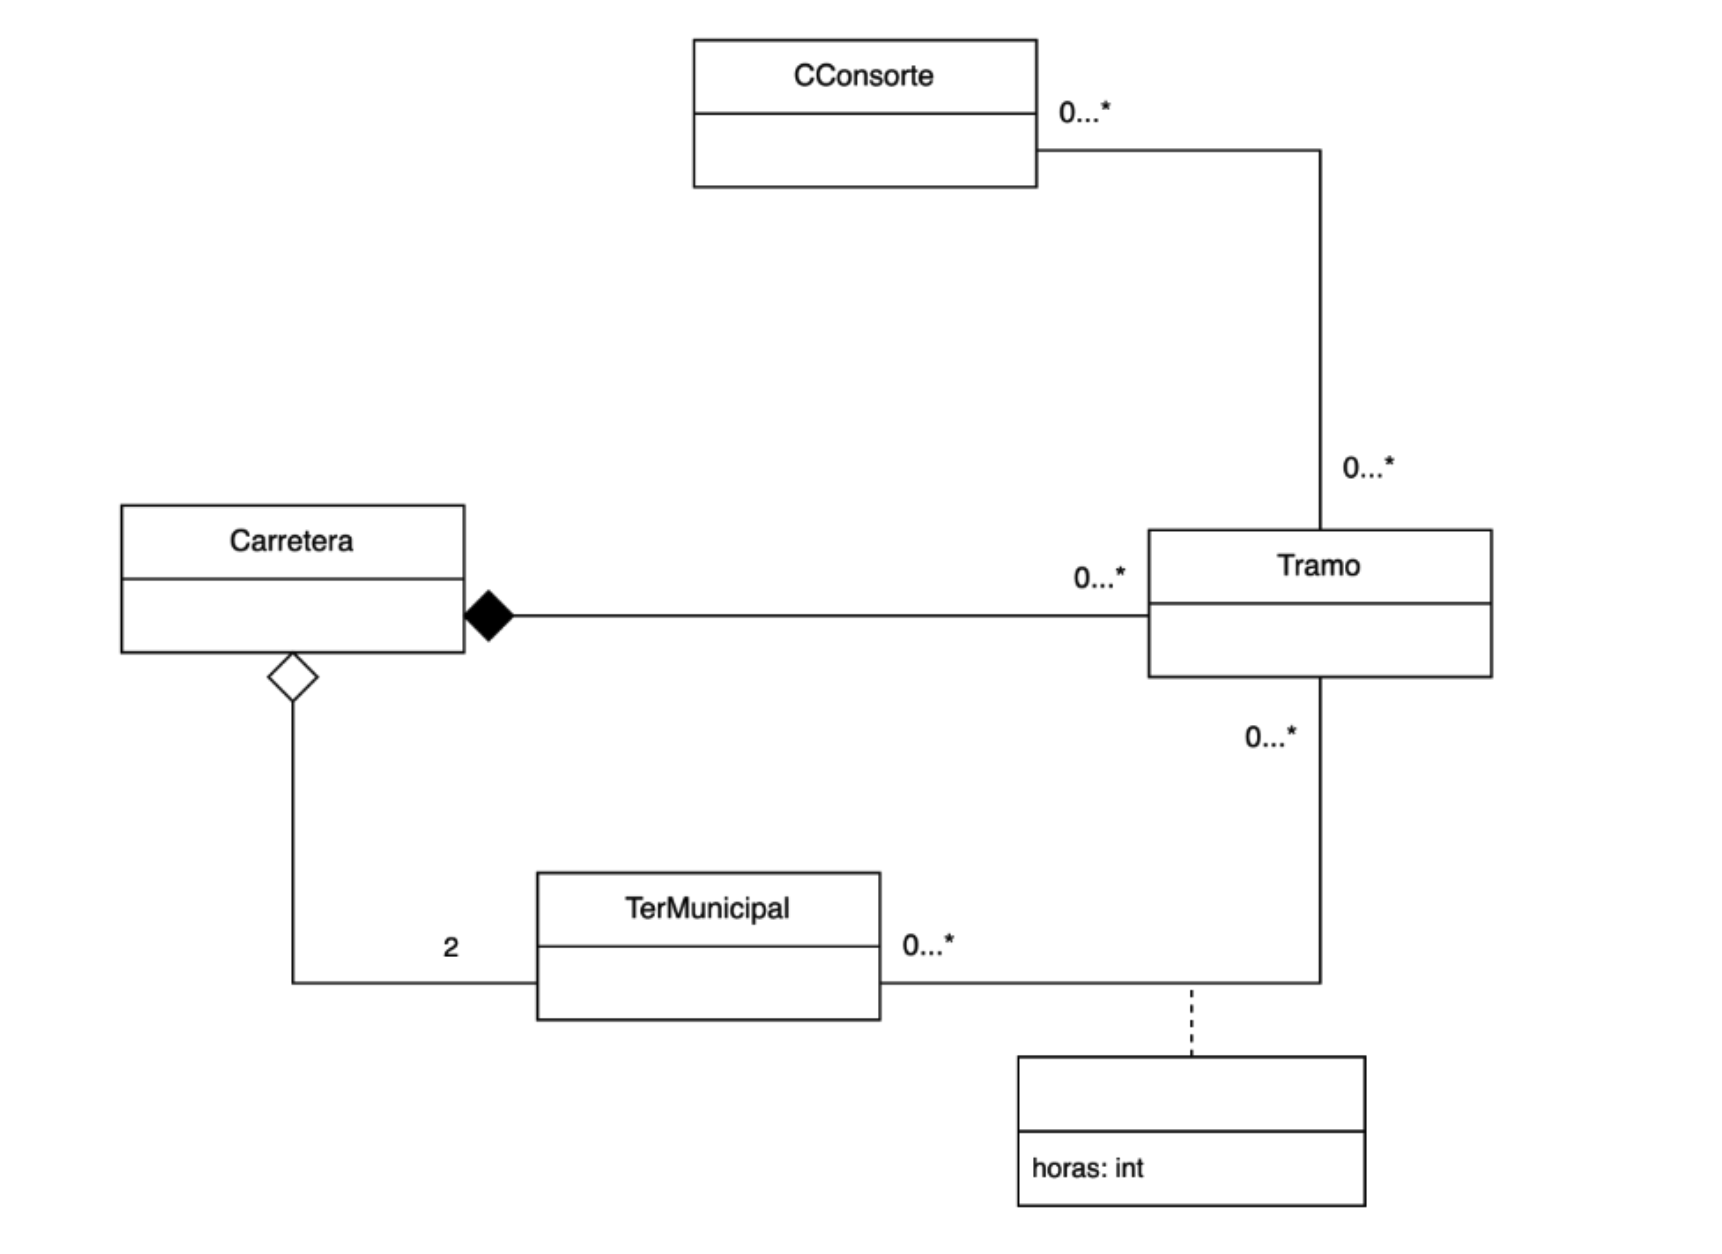
\includegraphics[width=\textwidth]{assets/Junio2023_1.png}
  \end{center}
  \caption{Diagrama de clase del ejercicio}
\end{figure}

\textbf{Relación Cconsorte - Tramo:}

Vemos que la relación entre Cconsorte y Tramos es una asociación muchos - muchos bidireccional, por tanto, la podemos implementar de dos maneras:
\begin{itemize}
  \item Mediante una clase de asociación que almacena los miembros imprescindibles para que se lleve a cabo la relación.
  \item Modificando las clases y añadiendo los miembros imprescindibles de la relación en cada una de las clases asociadas.
\end{itemize}
Nosotros implementaremos esta relación modificando las clases Cconsorte y Tramo.

\begin{minted}[breaklines]{C++}
class Cconsorte{
  public:
    //Alias del conjunto de objetos Tramos
    std::set<Tramo*>Tramos;
    void setTramo(Tramo&)noexcept;
    const Tramos& getTramos()const noexcept;
  private:
    Tramos tramos_;
};

class Tramo{
  public:
    //Alias del conjunto de objeto Cconsorte
    typedef std::set<Cconsorte*>Cconsortes;
    void setCconsorte(Cconsorte&)noexcept;
    const Cconsortes& getCconsortes()const noexcept;
  private:
    Cconsortes cconsortes_;
};
\end{minted}

\textbf{Relación Carretera - Tramo:}

La relación entre las clases Carretera y Tramo es una relación de composición 1-muchos, por tanto, no podemos implementarla mediante una herencia privada ya que la clase Carretera está formada por una serie de Tramos.
Esta relación son unidireccionales donde solo se alamcena la información de la relación en la clase compuesta (la que tiene el rombo).

\begin{minted}[breaklines]{C++}
class Carretera{
  public:
    //Alias del conjunto de objetos de Tramos
    std::set<Tramo>Tramos;
    Carretera(Tramo& );
    //tenemos que sobrecargar el operador < para poder ordenar las carreteras, ya que al ser un set de objetos y no de punteros no tenemos una implementación de dicho operador por defecto.
    friend bool operator < (const Carretera& , const Carretera&)noexcept;
  private:
    Tramos tramos_;
};
\end{minted}

\textbf{Relación Carretera - TerMunicipal:}

La relación entre las clases Carretera y TerMunicipal es de tipo agregación donde una instancia de Carretera se relaciona con dos instancias de TerMunicipal.
Las agregaciones se pueden implementar como asociaciones unidireccionales donde solo se almacena la información en la clase agregada (la que tiene el rombo).

\begin{minted}[breaklines]{C++}
class Carretera{
  public:
    //Miembros de la relación con la clase Tramo
    Carretera(Tramo& , TerMunicipal&, TerMunicipal&);
  private:
    Tramos tramos_;
    TerMunicipal t1, t2; //las dos instancias con las que se relaciona

};
\end{minted}

\textbf{Relación TerMunicipal - Tramo:}

Vemos que esta relación es del tipo asociación pero contiene un atributo de enlace, al ser las dos multiplicidad muchos - muchos la manera más fácil de implementar la relación es mediante una clase de asociación donde se alamcenará los miembros imprescindibles para que se lleve a cabo la relación.

\begin{minted}[breaklines]{C++}
class TerMunicipal_Tramo{
  public:
    //Alias del diccionario TerMunicipal - horas
    typedef std::map<TerMunicipal*,int>TerMunicipales;
    //Alias del diccionario Tramos - horas
    typedef std::map<Tramo*,int>Tramos;
    //Alias de los diccionarios de la clase 
    typedef std::map<Tramo*,TerMunicipales>TramosTer;
    typedef std::map<TerMunicipal*,Tramos>TerTramos;

    void setTerMunicipalTramo(TerMunicipal&, Tramo&, int)noexcept;
    void setTerMunicipalTramo(Tramo&, TerMunicipal&, int)noexcept;

    //observaores: como pueden no haber instancias, devolvemos una copia
    TerMunicipales getTerMunicipales(Tramo&)const noexcept;
    Tramos getTramos(TerMunicipal&)const noexcept;
  private:
    TerMunicipales directa_;
    Tramos inversa_;
};
\end{minted}
\newpage
\underbar{\textbf{\large Ejercicio 2:}} Sea este esquema:
\begin{figure}[h]
  \begin{center}
    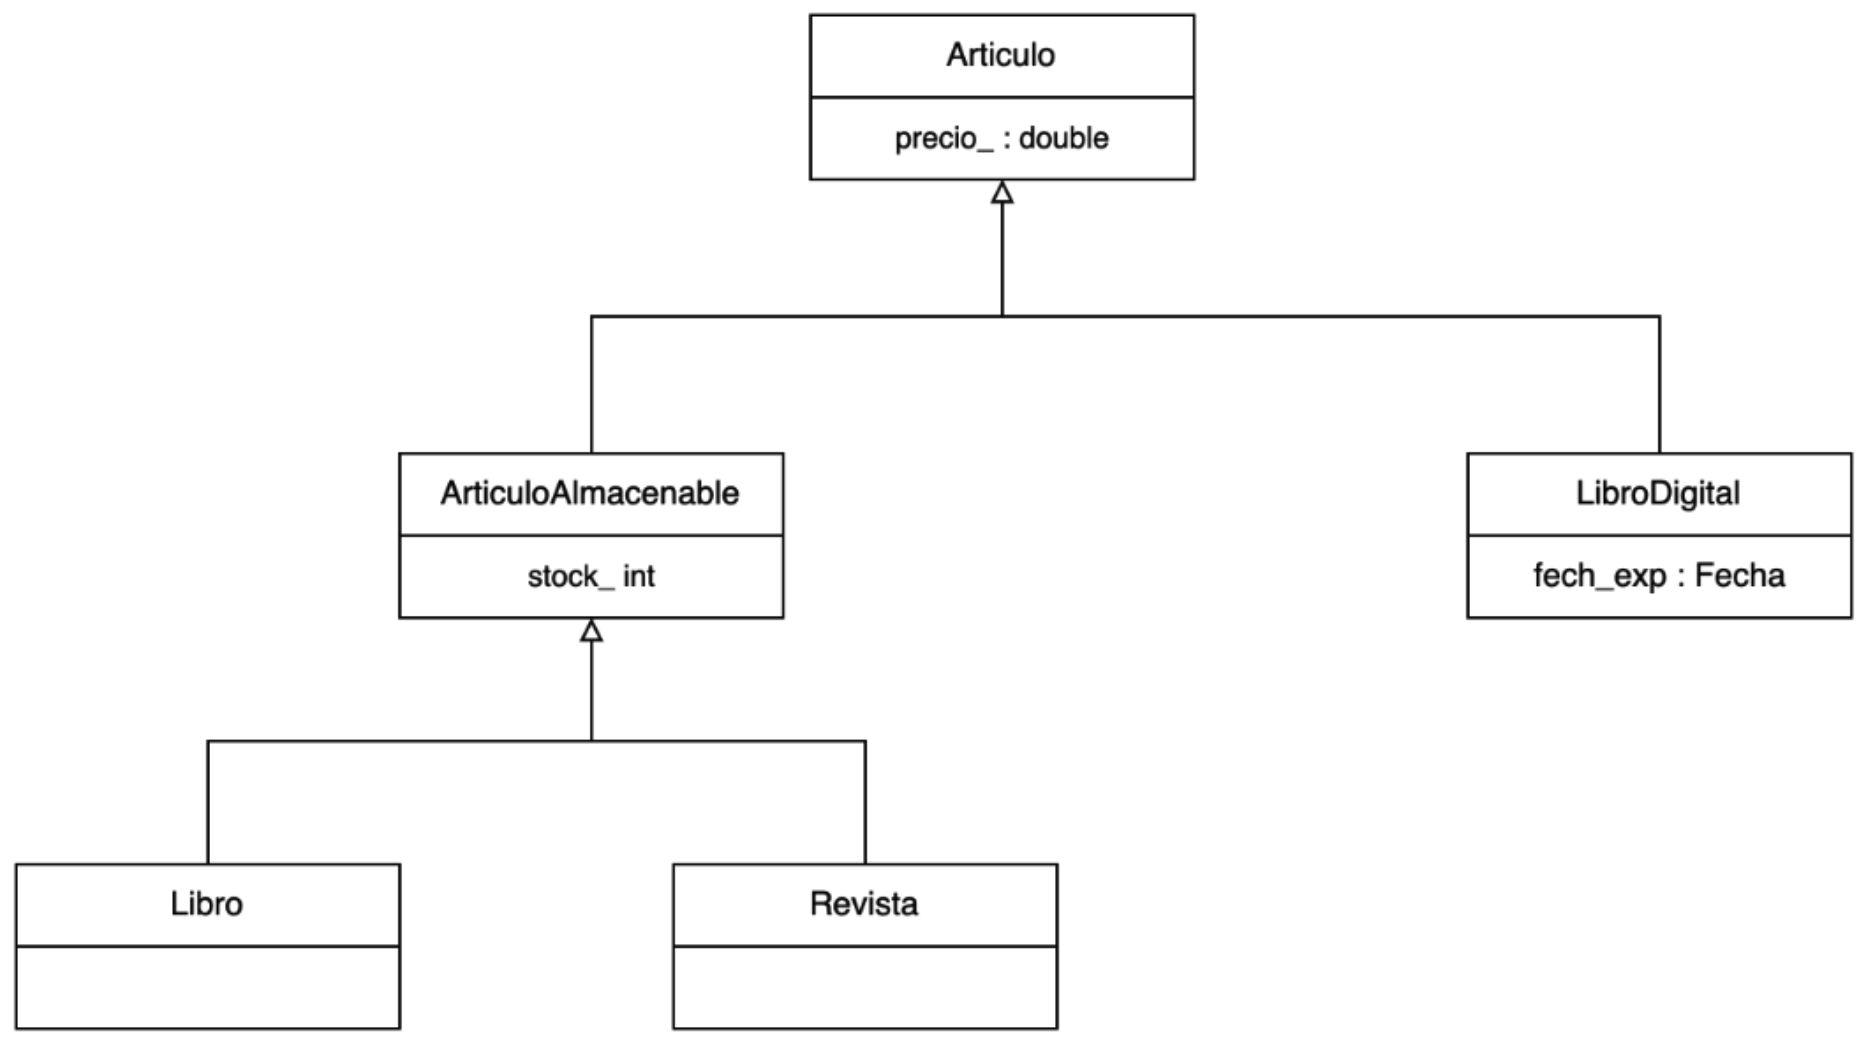
\includegraphics[width=\textwidth]{assets/Junio2023_2.png}
  \end{center}
\end{figure}

\begin{enumerate}
  \item Añade otra clase al esquema llamada DiscoDigital que contiene, al igual que LibroDigital, la fecha de expiración del DiscoDigital. Modifique el diagrama de acuerdo a esto.
\begin{minted}[breaklines]{C++}
class Articulo{
    double precio_;
  public:
    Articulo(double p):precio_(p){}
};

class ArticuloAlmacenable : public Articulo{
    int stock_;
  public:
    ArticuloAlmacenable(int s, double p):Articulo(p),stock_(s){}
};

class LibroDigital : public Articulo{
    Fecha fech_exp;
  public:
    LibroDigital(Fecha f, double p):Articulo(p),fech_exp(f){}
};

class Libro : public ArticuloAlmacenable{};
class Revista: public ArticuloAlmacenable{};
//Clase nueva que nos piede el ejercicio
class LibroDigital : public Articulo{
    Fecha f_expir_;
  public:
    LibroDigital(Fecha f, double p):Articulo(p),f_expir_(f){}
}
\end{minted}
  \item En esta nueva clase tenemos canciones. Se requiere saber en todo momento el número de canciones que tiene cada disco con el método observador nCancion()const.

  Un disco va a estar formado por una serie de canciones, como mínimo vamos a tener una canción. Por tanto, como no hay dependencia de existencia podemos implementarlo mediante una asociación a 1..muchos.
\begin{minted}[breaklines]{C++}
  class LibroDigital : public Articulo{
    Fecha f_expir_;
  public:
    LibroDigital(Fecha f, double p, Cancion& c):Articulo(p),f_expir_(f){
      setCanciones(c);
    }
    //Alias del conjunto de canciones del disco
    typedef std::set<Cancion*>Canciones;
    inline void setCanciones(Cancion&c )noexcept{
      canciones_.insert(&c);
    }
    inline const Canciones& getCanciones()const noexcept{
      return canciones_;
    }
  private:
    Canciones canciones_;
};
\end{minted}
  \item Implementa la clase Canción sabiendo que una canción pertenece a un solo disco, es necesario saber el número de canciones que tenemos en cada disco.

  Como bien nos dice una canción solo pertenece a un disco, por tanto, vamos a tener una relación de asociación 1 - 1..muchos como hemos comentado anteriormente.

\begin{minted}[breaklines]{C++}
class Cancion{
  public:
    inline void setDiscoDigital(DiscoDigital& disco)noexcept{
      discodigital_ = &disco;
    }
    inline const DiscoDigital& getDiscoDigital() const noexcept{
      return discodigital_;
    } 
  private:
    DiscoDigital discodigital_;
};
\end{minted}
\end{enumerate}
\newpage
\underbar{\textbf{\large Ejercicio 3:}}
\begin{enumerate}
  \item Para la figura anterior, implementar una función que te permita saber el número de Artículos (Revista, Libro, LibroDigital) que es menor que un precio dado, utilizando una estructura tipo EsBarato:

  Este método va a devolver un entero que por defecto será 0, y recibe por parámetros el conjunto de artículos a comprobar junto con el precio mínimo que tienen que superar, además dentro de la clase Articulo vamos a declarar el objeto a función EsBarato.
\begin{minted}[breaklines]{C++}
class Articulo{
  double precio_;
  public:
    //...
    inline const double getprecio()const noexcept{return precio_;}
    struct EsBarato{
      bool operator () (const Articulo& a, double precio){
        return a.precio_ < precio;
      }
    };
};

size_t ArticulosBaratos(const std::vector<Articulo*>& articulos, double precioMinimo){
  //variable que contendrá el número de articulos que son baratos
  size_t articulosbaratos = 0;
  //Definimos el objeto a funcion
  Articulo::EsBarato esbarato;

  //recorremos el conjunto de articulos comprobando si son baratos o no 
  for(const auto& a : articulos){
    if(esbarato(*a,precioMinimo)) articulosbaratos++;
  }
  return articulosbaratos;
}
\end{minted}
  \item El apartado anterior pero miramos solo los Libros y usando la forma Lambda.

  Ahora este método contará solamente los artículos que son Libros, por tanto, tendremos que convertir un objeto de tipo Articulo a un objeto de tipo Libro, lo haremos mediante dynamic\_cast para poder realizar dicha conversión ya que es de arriba - abajo.
\begin{minted}[breaklines]{C++}
size_t LibrosBaratos(const std::vector<Articulo*>& articulos, double precioMinimo)
{
  //Definimos la variable
  size_t librosbaratos = 0;
  //Creamos la función Lambda
  auto EsBarato = [precioMinimo](Articulo* a){
    //solo contamos los libros
    if(Libro* l = dynamic_cast<Libro*>(a)){
      return l!=nullptr && l->getprecio() < precioMinimo;
    }
  }
  //recorremos el vector de articulos
  for(const auto& a : articulos){
    //comprobamos si es barato o no
    if(EsBarato(a))librosbaratos++;
  }
  return librosbaratos;
}
\end{minted}
  \item Devolver el lista de articulos que hay que reponer, dado un lista de punteros a Articulo y un stock minimo.

  Ahora vamos a crear un método que va a devolver un conjunto (vector) de los articulos que tendrán que ser repuestos, esa comprobación podemos hacerlo o bien con un objeto a función o con una función Lambda que nos comprueben el stock del articulo con el stock minimo dado por parámetro.

  Además solamente podemos obtener el stock de los ArticulosAlmacenables por tanto, al recibir un vector de tipo Articulo, tenemos que convertir dichos objetos al tipo ArticuloAlmacenable y acceder al método observador \texttt{getstock()}

\begin{minted}[breaklines]{C++}
class ArticuloAlmacenable : public Articulo{
    int stock_;
  public:
    ArticuloAlmacenable(int s, double p):Articulo(p),stock_(s){}
    inline int getstock()const noexcept{return stock_;}
};
std::vector<Articulo*> ReponeArticulos(const std::vector<Articulo*>& articulos, int stockMinimo)
{
  //creamos el vector a devolver
  std::vector<Articulo*>articulosAreponer
  //Creamos la función Lambda
  auto Reponer = [stockMinimo](Articulo* a){
    //convertimos los articulos en ArticulosAlmacenables para ver su stock
    if(ArticuloAlmacenable* AA = dynamic_cast<ArticuloAlmacenable*>(a)){
      return AA!=nullptr && AA->getstock() < stockMinimo;
    }
  }
  //Ahora recorremos el vector de articulos comprobando su stockMinimo
  for(const auto& a : articulos){
    if(Reponer(a))articulosAreponer.push_back(a);
  }
  return articulosAreponer;
}
\end{minted}
\end{enumerate}
\newpage
\underbar{\textbf{\large Ejercicio 4:}} Sea la clase Matriz:
\begin{center}
  \begin{lstlisting}[frame = single]
class Matriz{
  public:
    Matriz(size_t m = 10, size_t n= 10, double y = 0.0): 
      m(m), n(n), x(m*n,y){}

  private:
    size_t m, n;
    std::valarray<double> x;
};
  \end{lstlisting}
\end{center}

\begin{enumerate}
  \item Implementela con el uso de templates para cuaquier de tipo de dato, por omisión esta plantilla será tipo double. La matriz está compuesta por F(Fila), C(Columna). Con F y C por omision 10. El constructor por defecto es del tipo por omision T. Crea un objeto de tipo Matriz que sea :
  \begin{itemize}
    \item Una matriz m1 de tipo base inicializada con los datos por omisión.
    \item Una matriz m2 de tipo double de 10 x 10 con elementos 1.
    \item Una matriz m3 de tipo double y 3 x 4 con elementos 0.
  \end{itemize}
  Qué pasaría si hicieramos \texttt{m1 = m2; m2 = m3; }

  Escribe la declaración de un \texttt{ostream << ()} para cualquier tipo de plantilla.
\end{enumerate} 

Para poder asignar matrices como estas pueden tener dimensiones diferentes debemos de implementar tanto el constructor de copia como el operador de asignación por copia, para poder asignar matrices a otras sin que se pierda información.

\begin{minted}[breaklines]{C++}
template <typename T = double>
class Matriz{
  public:
    Matriz(T m = 10, T n = 10, T y = 0.0):
      m_(m),n_(n),x_(m*n , y){}

    //Constructor por copia
    Matriz(const Matriz<T>& other):m_(other.m_),n_(other.n_):x_(other.x_){}

    //operador de asignación por copia
    Matriz<T>& operator = (const Matriz<T>& other){
      if(this!=&other){//evitamos la autoasignación
        //comprobamos que tengan el mismo número de filas y columnas
        if(m_ != other.m_ || n_ !=other.n_){
          //cambiamos los tamaños
          m_ = other.m_;
          n_ = other.n_;
          //reajustamos el tamaño de la matriz
          x_.resize(m_*n_);
        }
        return *this;
      }
    }
    //operador de inserción en flujo
    friend std::ostream& operator << (std::ostream& , const Matriz<T>& )noexcept;
  private:
    T m_,n_;
    std::valarray<T> x_;
};

\end{minted}